\documentclass[12pt,a4paper]{article}
\usepackage[polish]{babel}
\usepackage[utf8]{inputenc}
\usepackage[T1]{fontenc}
\usepackage{amsmath}
\usepackage{amsfonts}
\usepackage{amssymb}
\usepackage{graphicx}
\usepackage{listings}
\usepackage{xcolor}
\usepackage{float}
\usepackage{caption}
\usepackage{subcaption}

\title{Sprawozdanie z analizy algorytmów sortowania}
\author{Jan Mikołajczyk}
\date{28.10.2025}

\begin{document}

\maketitle

\section{Wprowadzenie}
W ramach listy zadań zaimplementowano i przeanalizowano sześć algorytmów sortowania: Insertion Sort, zmodyfikowany Insertion Sort, Merge Sort, trójdrożny Merge Sort, Heap Sort oraz trójdrożny Heap Sort. Analiza obejmowała porównanie liczby porównań, przypisań oraz czasu wykonania dla różnych rozmiarów danych.

\section{Analiza kodów źródłowych}

\subsection{Kluczowe fragmenty kodu}

\subsubsection{Insertion Sort z modyfikacją}
\begin{lstlisting}[language=C++,caption=Modyfikacja Insertion Sort]
        //...
        while(j>=0 && tab[j]>x){
            comparisons += 2;
            tab[j+1]=tab[j];
            assignments++;
            j--;
        }
        comparisons += (j>=0 ? 2 : 1);
        tab[j+1]=x;
        assignments++;

        int k=i;
        assignments++;

        while(k>=0 && tab[k]>y){
            comparisons += 2;
            tab[k+1]=tab[k];
            assignments++;
            k--;
        }
        //...
\end{lstlisting}
\textbf{Opis:} Ten fragment jest kluczowy dla działania zmodyfikowanego algorytmu Insertion Sort, ponieważ odpowiada za właściwe wstawienie dwóch kolejnych elementów (x i y) w odpowiednie miejsca w częściowo posortowanej tablicy. Pętle while realizują przesuwanie większych elementów w prawo, tak aby zachować porządek rosnący i jednocześnie umożliwić wstawienie analizowanych wartości.

\subsubsection{Trójdrożny Merge Sort}
\begin{lstlisting}[language=C++,caption=Merge Sort z trzema podtablicami]
void MERGE_3TAB(int leftTab[],int middleTab[],int rightTab[],
      int tab[], int leftSize,int middleSize, int rightSize){
    int i=0,l=0,m=0,r=0;
    while(l<leftSize && m<middleSize && r<rightSize){
        comparisons += 3;
        comparisons += 2;
        if(leftTab[l]<middleTab[m] && leftTab[l]<rightTab[r]){
            tab[i]=leftTab[l];
            i++; l++;
        }
        // ... 
    }
}
\end{lstlisting}
\textbf{Opis:} Algorytm dzieli tablicę na trzy części zamiast dwóch, co teoretycznie powinno zmniejszyć głębokość rekurencji. Jednakże zwiększa to złożoność operacji scalania.

\subsubsection{Trójdrożny Heap Sort}
\begin{lstlisting}[language=C++,caption=Kopiec trójkowy]
void HEAPIFY_TRIPLE(int tab[], int n, int i){
    int left=3*i+1;
    int middle=3*i+2;
    int right=3*i+3;
    int largest=i;
    
    if(left<n&&tab[left]>tab[largest]){
        largest=left;
    }
    if(middle<n&&tab[middle]>tab[largest]){
        largest=middle;
    }
    if(right<n&&tab[right]>tab[largest]){
        largest=right;
    }
    // ... 
}
\end{lstlisting}
\textbf{Opis:} W tej implementacji każdy węzeł ma troje dzieci zamiast dwojga, co zmniejsza wysokość kopca ale zwiększa liczbę porównań przy przywracaniu własności kopca.

\section{Porównanie działania algorytmów}

\subsection{Metodologia badań}
Badania przeprowadzono dla tablic o rozmiarach: 1000, 2500, 5000, 10000, 25000, 50000, 75000 i 100000 elemententowych. Dla każdego rozmiaru tablicy wygenerowano liczby z przedziału od 1-1000.

\subsection{Wyniki pomiarów}

\begin{table}[H]
\centering
\caption{Porównanie algorytmów dla 1000 elementów}
\begin{tabular}{|l|c|c|c|}
\hline
Algorytm & Porównania & Przypisania & Czas [ms] \\
\hline
HEAP SORT & 48 025 & 48 609 & 0.1818 \\
TRIPLE HEAP SORT & 46 249 & 34 375 & 0.1705 \\
MERGE SORT & 42 876 & 23 948 & 0.1798 \\
MERGE SORT MODE & 30 552 & 14 052 & 0.1135 \\
INSERTION SORT & 504 529 & 254 264 & 0.6616 \\
INSERTION SORT MOD & 506 542 & 255 755 & 0.7087 \\
\hline
\end{tabular}
\end{table}

\begin{table}[H]
\centering
\caption{Porównanie algorytmów dla 10000 elementów}
\begin{tabular}{|l|c|c|c|}
\hline
Algorytm & Porównania & Przypisania & Czas [ms] \\
\hline
HEAP SORT & 645 410 & 667 409 & 2.4168 \\
TRIPLE HEAP SORT & 607 572 & 462 621 & 1.5249 \\
MERGE SORT & 562 682 & 307 228 & 2.1749 \\
MERGE SORT MODE & 385 660 & 186 004 & 0.9971 \\
INSERTION SORT & 50 364 071 & 25 202 037 & 74.6443 \\
INSERTION SORT MOD & 50 384 091 & 25 217 022 & 69.9895 \\
\hline
\end{tabular}
\end{table}

\begin{table}[H]
\centering
\caption{Porównanie algorytmów dla 100000 elementów}
\begin{tabular}{|l|c|c|c|}
\hline
Algorytm & Porównania & Przypisania & Czas [ms] \\
\hline
HEAP SORT & 8 118 770 & 8 505 064 & 21.2176 \\
TRIPLE HEAP SORT & 7 548 520 & 5 819 453 & 18.9844 \\
MERGE SORT & 6 954 467 & 3 737 852 & 32.2100 \\
MERGE SORT MODE & 4 594 011 & 2 315 761 & 14.3170 \\
INSERTION SORT & 4 989 083 795 & 2 494 741 899 & 5967.74 \\
INSERTION SORT MOD & 4 989 283 741 & 2 494 891 958 & 6106.96 \\
\hline
\end{tabular}
\end{table}

\section{Wnioski z przeprowadzonych obserwacji}

Na podstawie analizy wyników pomiarów dla różnych rozmiarów danych wejściowych (1000, 10000, 100000 elementów) można wyciągnąć następujące wnioski:

\subsection{Wydajność czasowa}
\begin{itemize}
\item Algorytmy \textbf{MERGE\_SORT\_MODE} i \textbf{TRIPLE\_HEAP\_SORT} wykazują najlepszą wydajność czasową dla wszystkich badanych rozmiarów danych
\item Algorytmy insertion sort (\textbf{INSERTION\_SORT} i \textbf{INSERTION\_SORT\_MOD}) są znacząco wolniejsze od pozostałych algorytmów, szczególnie dla dużych zbiorów danych (dla 100000 elementów czas wykonania przekracza 5 sekund)
\item Dla 100000 elementów różnica w czasie wykonania między najszybszym (\textbf{MERGE\_SORT\_MODE} - 14.32 ms) a najwolniejszym (\textbf{INSERTION\_SORT} - 5967.74 ms) algorytmem wynosi ponad 400-krotność
\end{itemize}
\subsection{Liczba operacji porównań}
\begin{itemize}
\item \textbf{MERGE\_SORT\_MODE} wykonuje najmniejszą liczbę porównań we wszystkich przypadkach testowych
\item Algorytmy insertion sort wykonują zdecydowanie najwięcej porównań.
\item Dla 100000 elementów \textbf{INSERTION\_SORT} wykonuje prawie 5 miliardów porównań, podczas gdy \textbf{MERGE\_SORT\_MODE} tylko około 4.6 miliona
\end{itemize}

\subsection{Liczba operacji przypisań}
\begin{itemize}
\item \textbf{MERGE\_SORT\_MODE} charakteryzuje się również najmniejszą liczbą przypisań
\item \textbf{TRIPLE\_HEAP\_SORT} wykonuje mniej przypisań niż standardowy \textbf{HEAP\_SORT}, co świadczy o jego optymalizacji
\item Algorytmy oparte na strukturze kopca (\textbf{HEAP\_SORT} i \textbf{TRIPLE\_HEAP\_SORT}) wykonują więcej przypisań niż algorytmy sortowania przez scalanie
\end{itemize}

\begin{figure}[H]
\centering
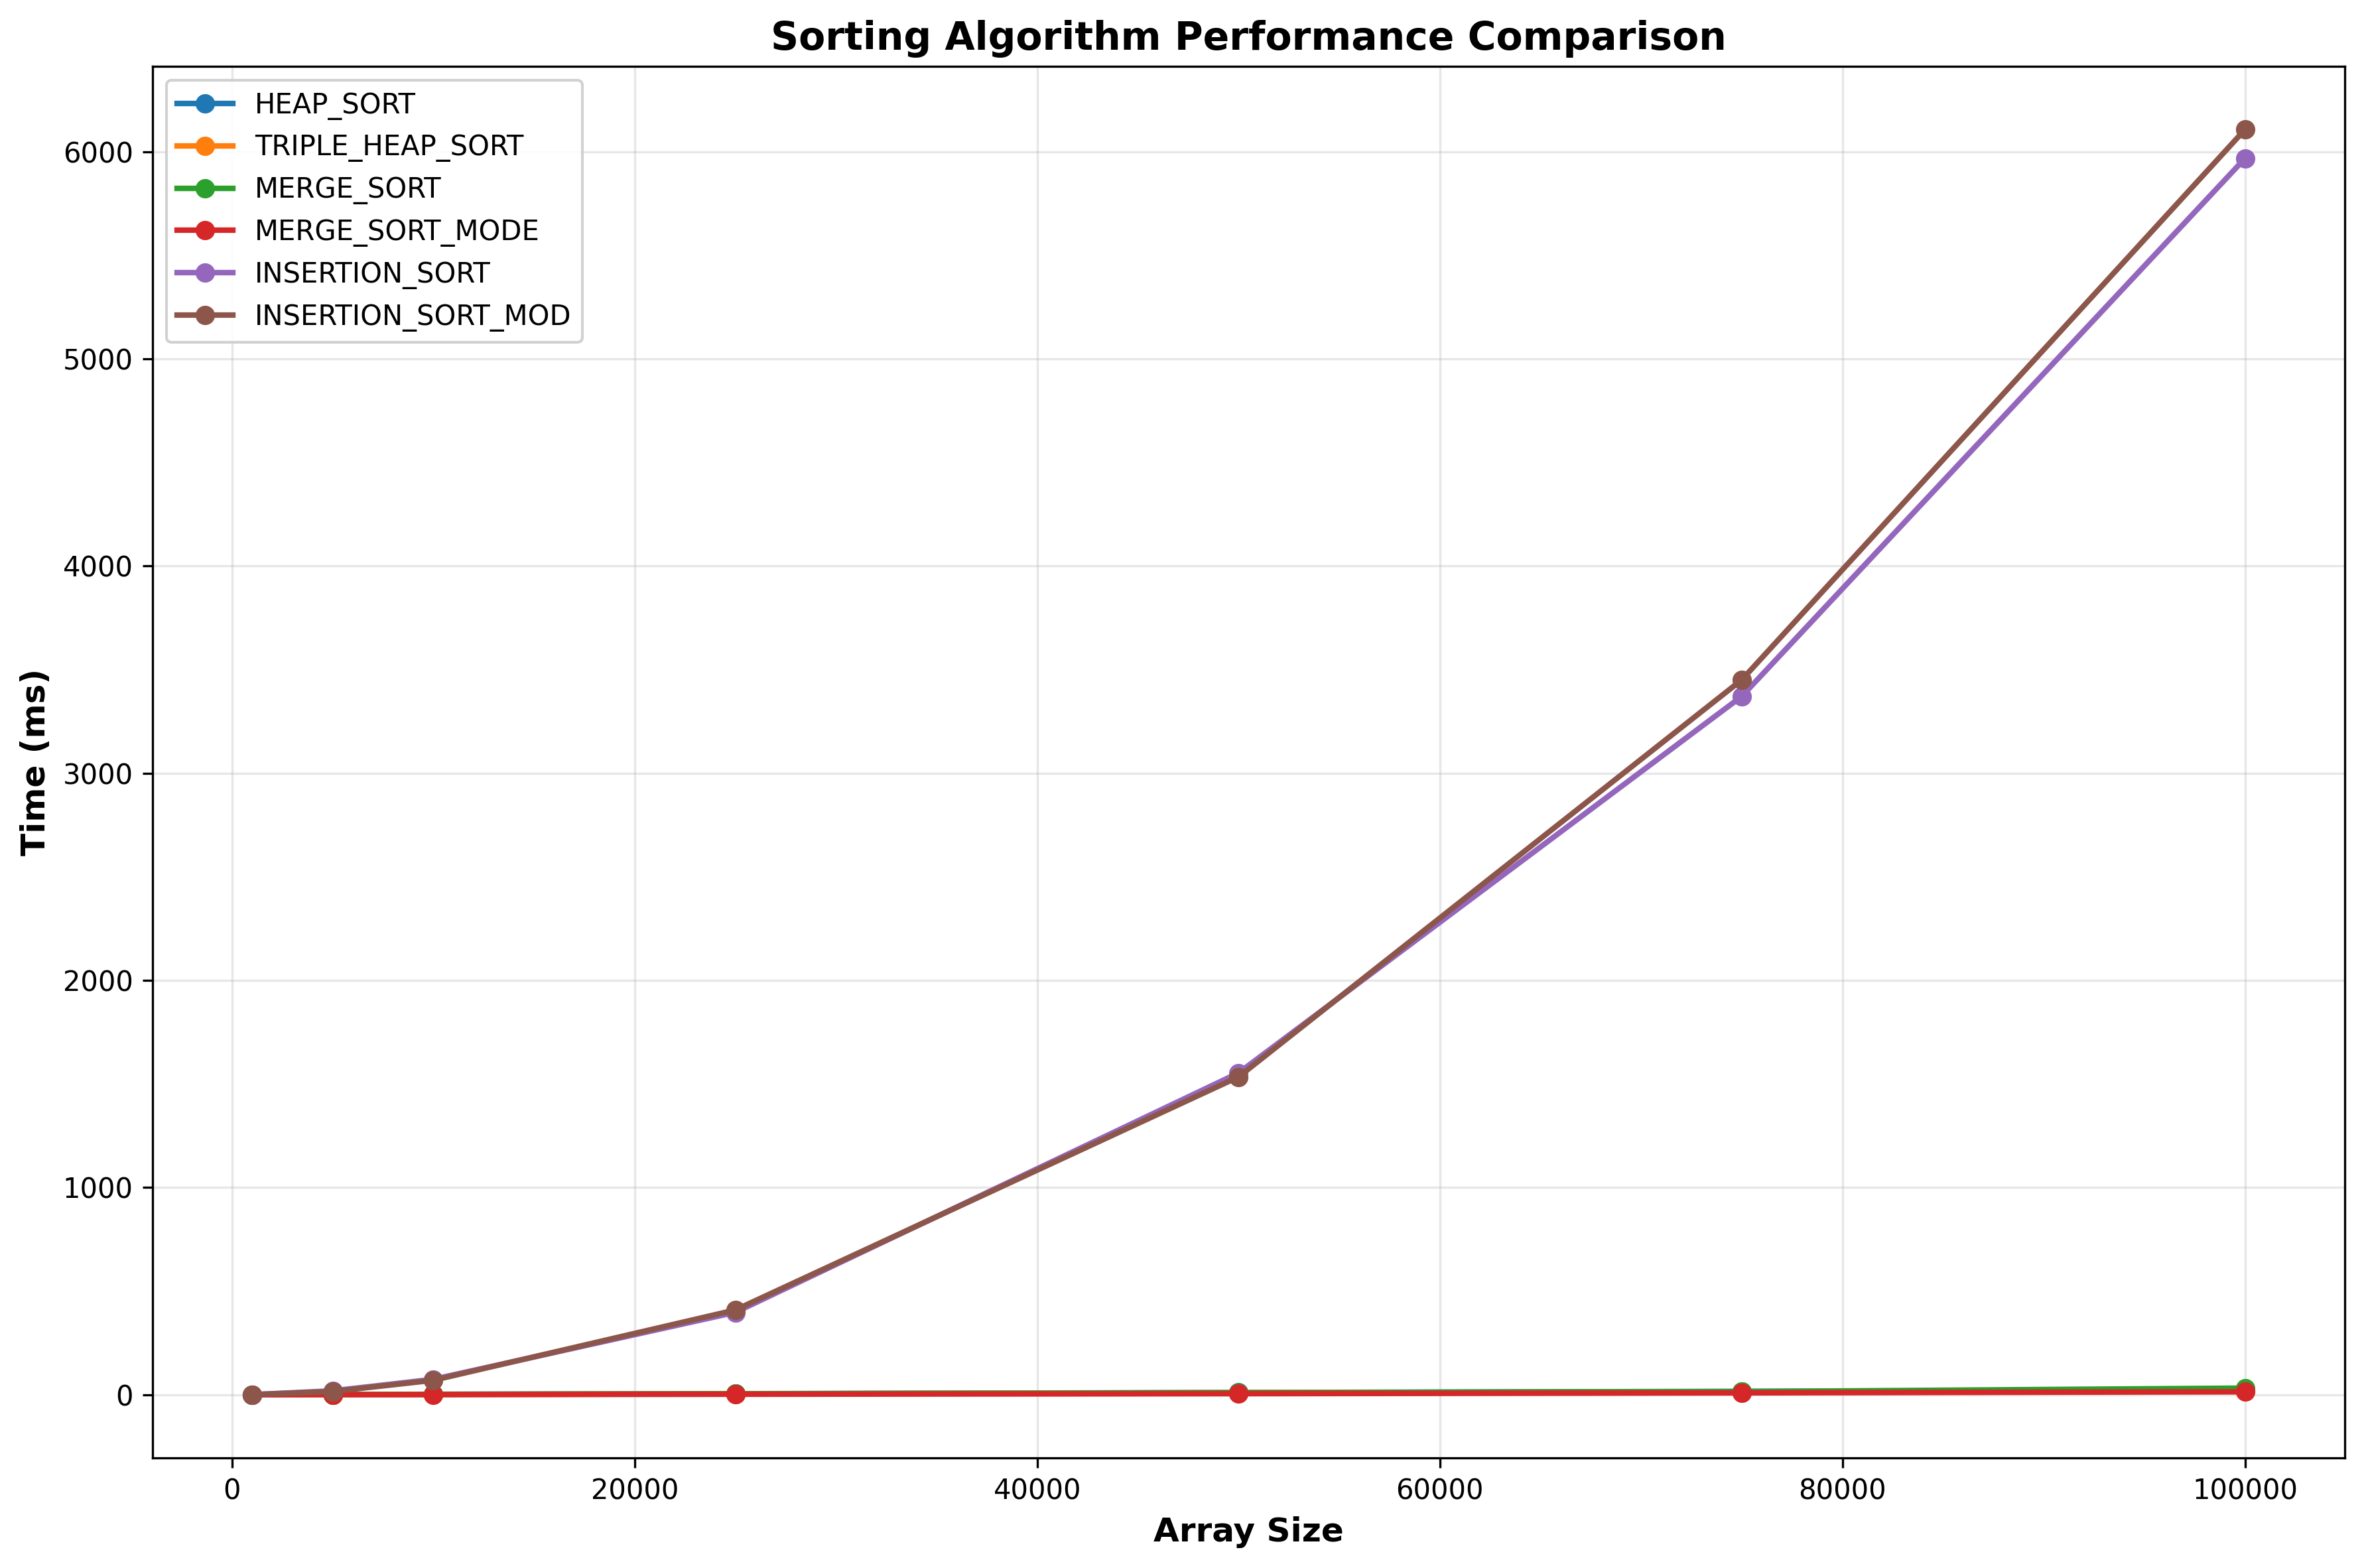
\includegraphics[width=0.8\textwidth]{algorithm_performance.png}
\caption{Porównanie czasu wykonania algorytmów dla różnych rozmiarów danych}
\end{figure}

\begin{figure}[H]
\centering
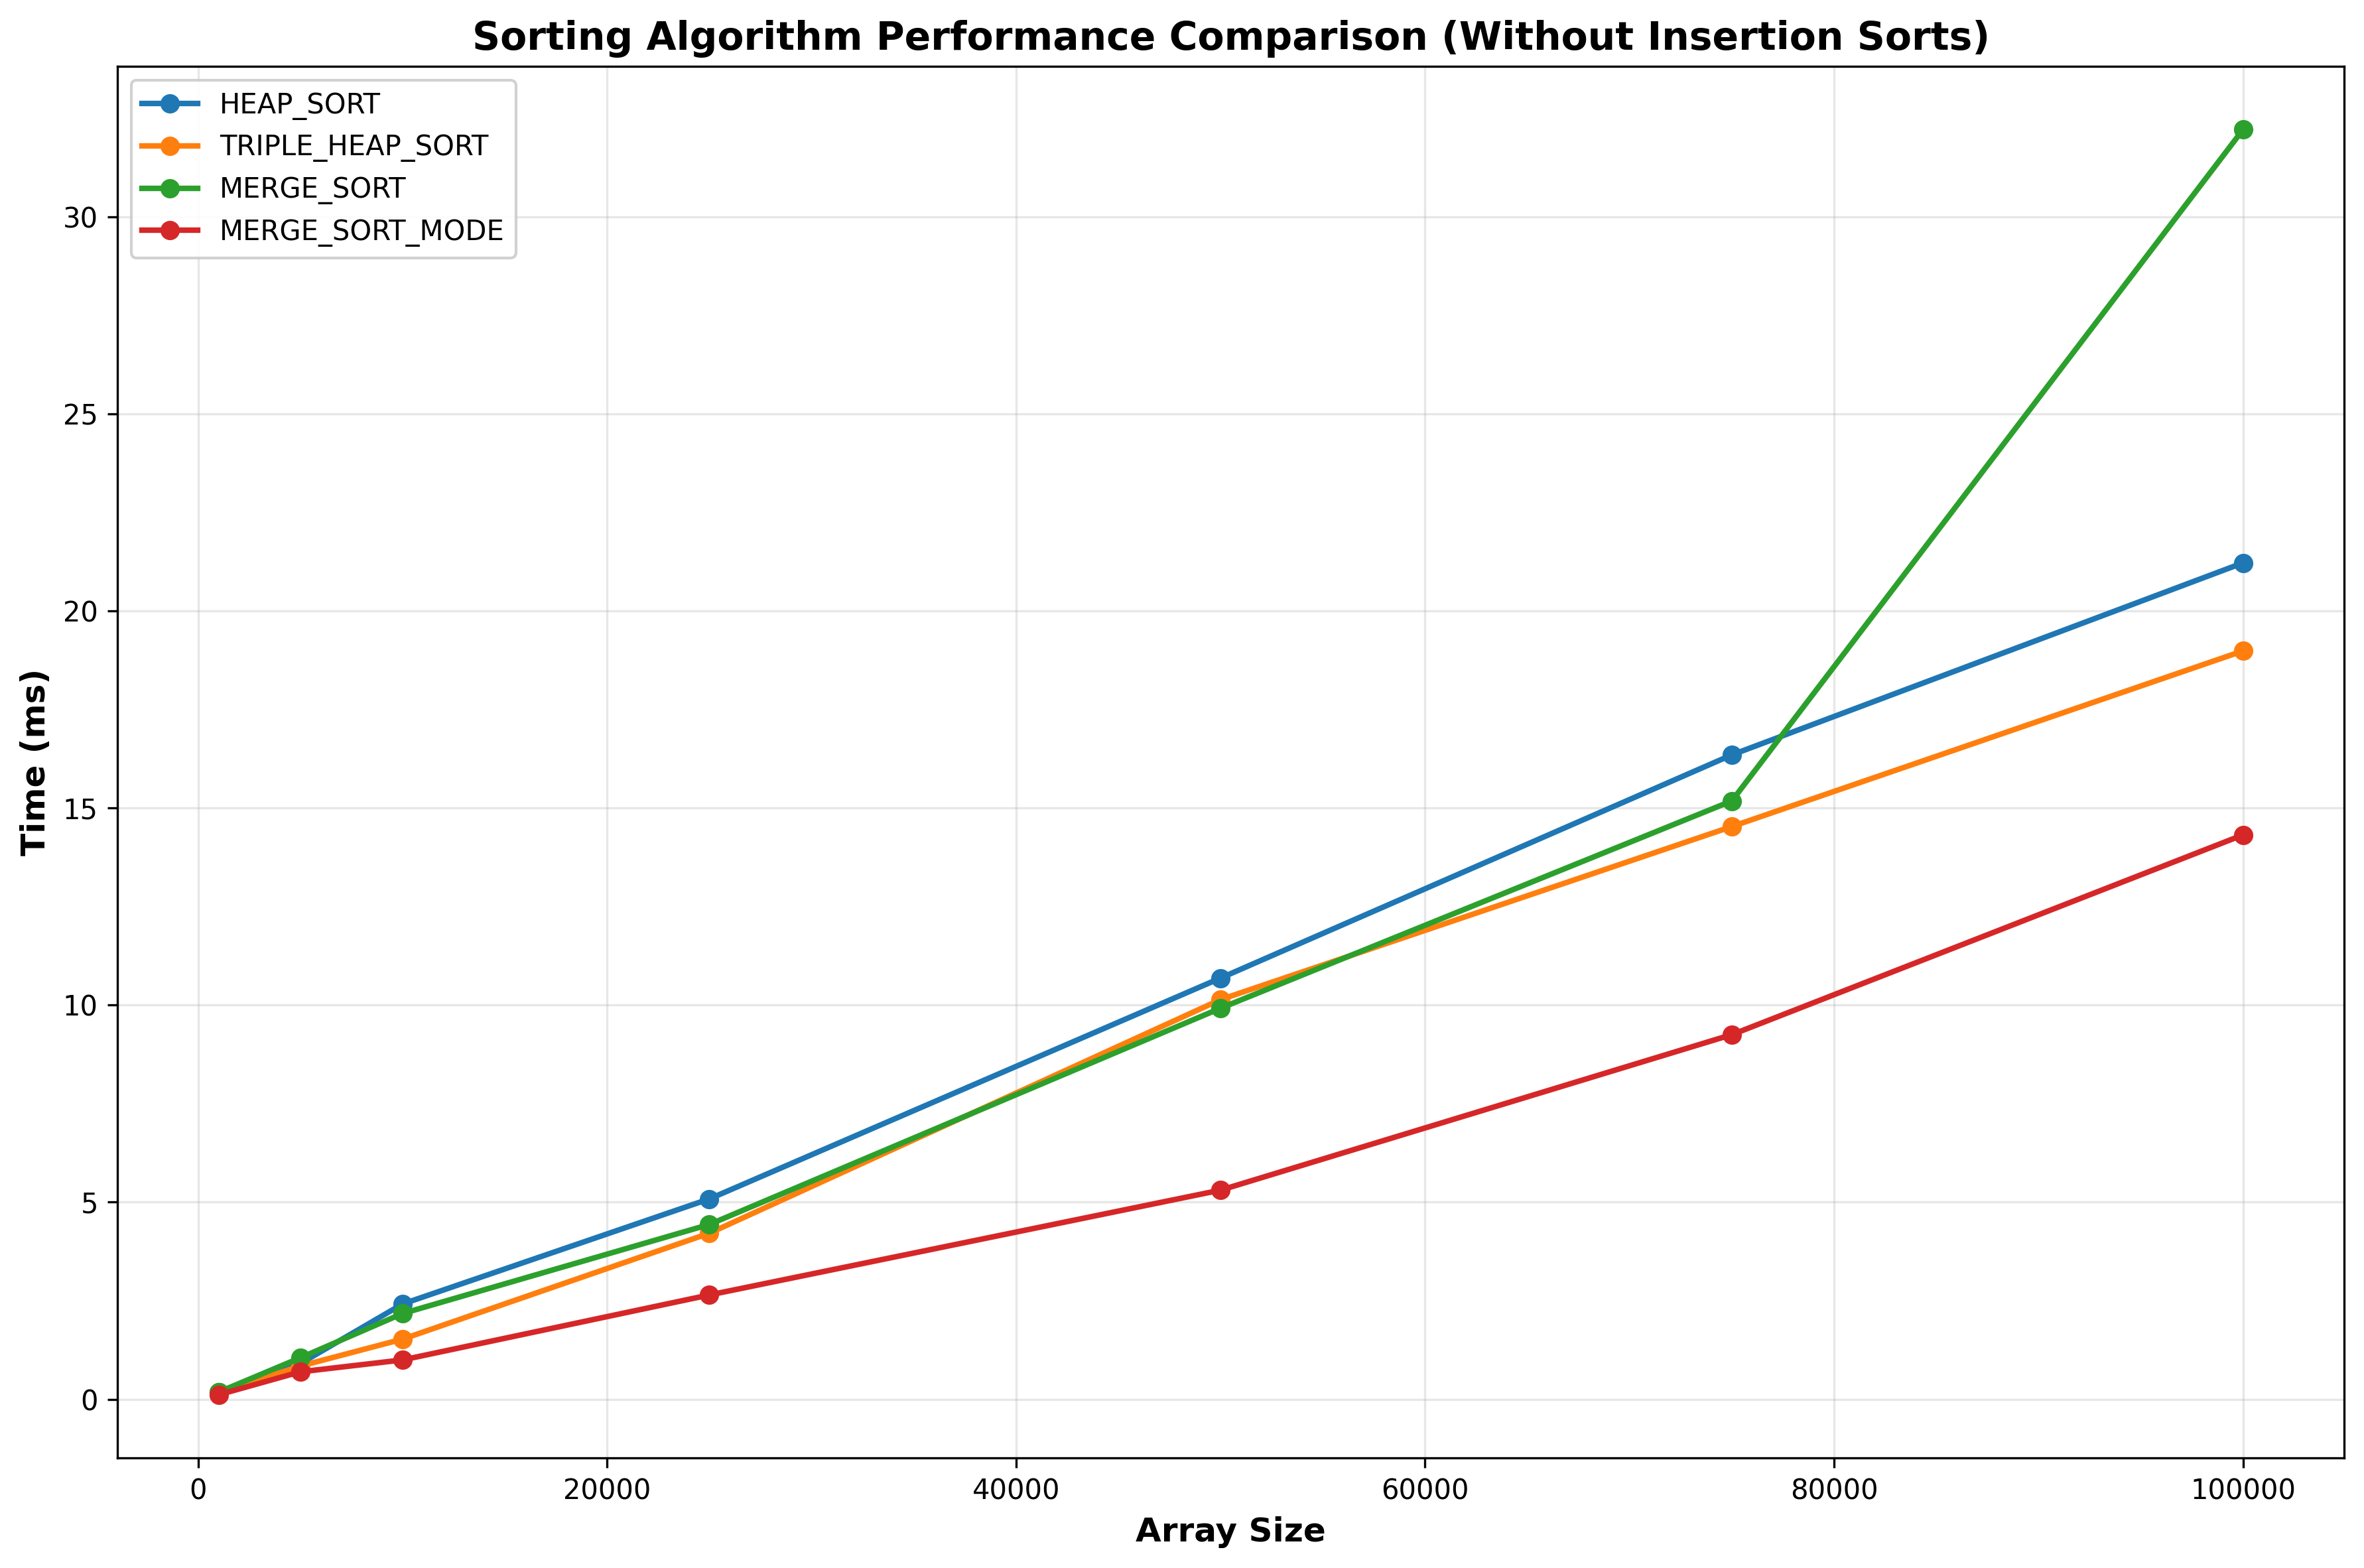
\includegraphics[width=0.8\textwidth]{algorithm_performance_no_insertion.png}
\caption{Porównanie czasu wykonania algorytmów dla różnych rozmiarów danych (bez insertion sort)}
\end{figure}

Z powyższych wykresów możemy zauważyć, że \textbf{TRIPLE\_HEAP\_SORT} i
\textbf{MERGE\_SORT\_MODE} są stosunkowo najszybsze (dla naszych próbek danych). Dokonajmy więc ich bliższego porównania.

\begin{figure}[H]
\centering
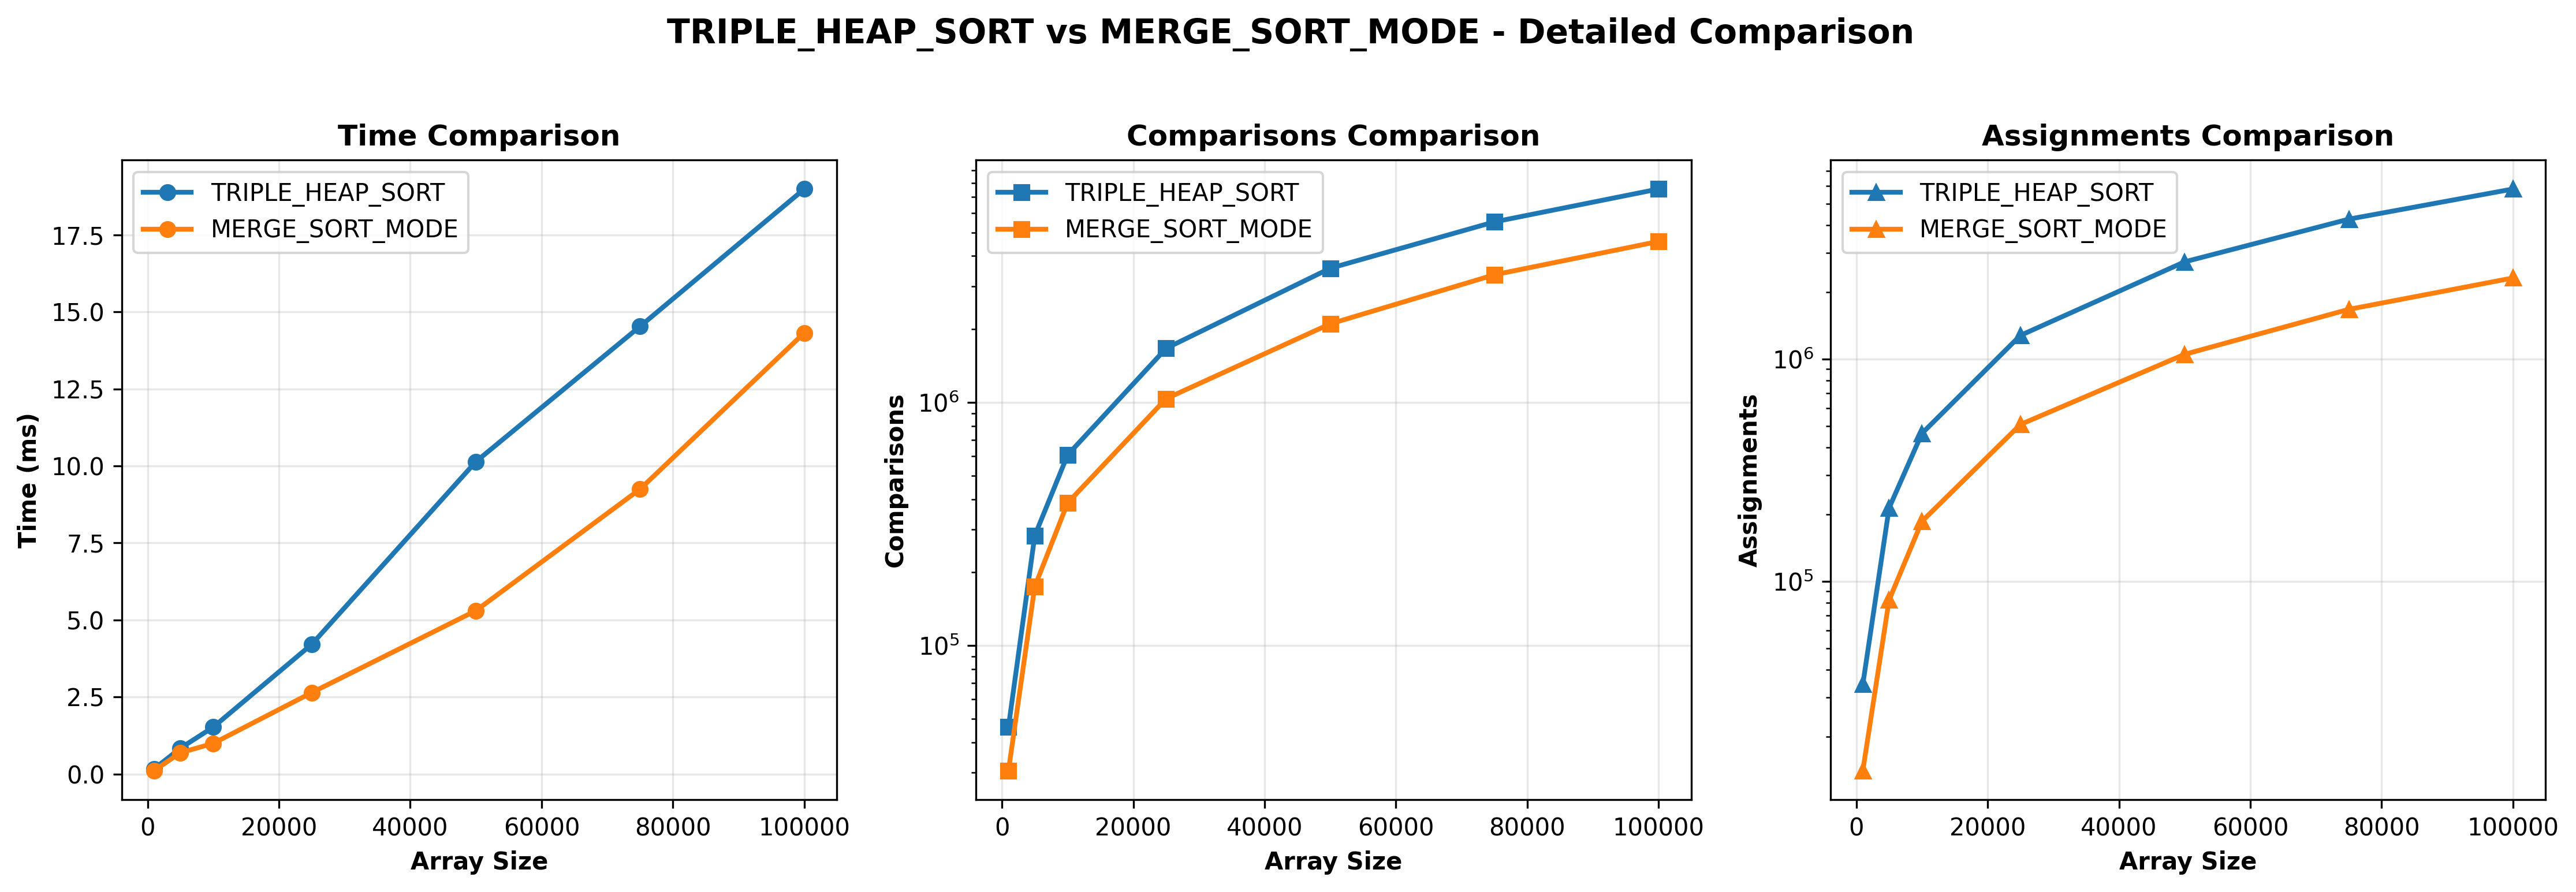
\includegraphics[width=0.8\textwidth]{best_algorithms_comparison.png}
\caption{}
\end{figure}

\section{Wnioski}

\subsection{Analiza efektywności}

\begin{enumerate}
\item \textbf{Algorytmy proste vs. zaawansowane:}  
Wyniki jednoznacznie pokazują, że dla małych zbiorów danych (np. 1000 elementów) różnice czasowe pomiędzy algorytmami nie są duże, jednak wraz ze wzrostem rozmiaru danych przewagę zyskują algorytmy o złożoności $O(n \log n)$.  
Dla tablic zawierających 100000 elementów, algorytmy \textbf{Insertion Sort} i jego modyfikacja są nawet ponad 400 razy wolniejsze od algorytmów opartych na scalaniu lub kopcu.

\item \textbf{Modyfikacje klasycznych algorytmów:}
\begin{itemize}
\item Modyfikacja \textbf{Insertion Sort} (z dwoma elementami jednocześnie) nie przyniosła istotnej poprawy efektywności — liczba porównań i przypisań wzrosła nieznacznie, a czas wykonania pozostał na podobnym poziomie jak w wersji klasycznej.
\item W przypadku \textbf{Trójdrożnego Merge Sort} zauważono spadek liczby porównań w stosunku do klasycznego Merge Sort, jednak kosztem większej liczby przypisań.
\item \textbf{Trójdrożny Heap Sort} okazał się korzystniejszy od klasycznego Heap Sort – wykonał mniej przypisań i porównań, co przełożyło się na krótszy czas działania, szczególnie dla większych danych.
\end{itemize}

\subsection{Podsumowanie}

Na podstawie przeprowadzonych eksperymentów można sformułować następujące wnioski końcowe:

\begin{itemize}
\item Najbardziej zrównoważonym algorytmem pod względem szybkości, liczby operacji oraz stabilności okazał się \textbf{Merge Sort Mode}.
\item \textbf{Triple Heap Sort} osiągnął bardzo dobre wyniki czasowe, stając się wydajniejszą alternatywą dla klasycznego Heap Sort, szczególnie przy dużych zbiorach danych.
\item Modyfikacje prostych algorytmów (np. Insertion Sort) nie przyniosły wymiernych korzyści i nie mają praktycznego zastosowania przy większych zbiorach danych.
\item Wybór optymalnego algorytmu zależy od kontekstu zastosowania:  
\begin{itemize}
\item dla małych zbiorów — prostsze algorytmy mogą być wystarczające,  
\item dla dużych danych — najlepsze wyniki uzyskują algorytmy o złożoności $O(n \log n)$, takie jak \textbf{Merge Sort Mode} lub \textbf{Triple Heap Sort}.
\end{itemize}


\end{document}